\clearpage
\twocolumn[{%
\subsection{Above chance against the tokens of the language seen}
\label{app:rq00_chance_vs_train_tokens}

\noindent\begin{minipage}[t]{0.485\textwidth}
\vspace{0pt}
\paragraph{Research Question.} \emph{Does a benchmark task clear chance once the model has seen enough of the task's language, and is that exposure or model size?}

\paragraph{Setup.} A cell is one (task, size, language setting) read at each of the ten evaluated tenths of the run. We place it at the number of tokens of the task's language that the checkpoint had seen. This number is the language's share of the mixture $\times$ the size's budget $\times$ the tenth. We use seed-1904 runs of every data build and ladder, 90M--1.7B, at $K \in \{1, 2, 8, 15, 30, 50\}$. The above-chance gate is applied per run.
\end{minipage}\hfill
\begin{minipage}[t]{0.485\textwidth}
\vspace{0pt}
\begin{rqfinding}
\textbf{1. Outside English, the share of cells above chance rises with every decade of the language's tokens from $10^{7}$ on.} But at matched tokens the larger model still clears chance more often. The share goes from 40 \% at $10^{7}$--$10^{8}$ tokens to 62 \% at $10^{10}$--$10^{11}$, and at $10^{8}$--$10^{9}$ tokens it is 40 \% at 90M against 60 \% at 1.7B: exposure is necessary, not sufficient. (Figure~\ref{fig:app_rq00_chance_vs_train_tokens}.)
\\
\\
\textbf{2. Pooled over every language the curve peaks at $10^{8}$--$10^{9}$ tokens and falls after, because the top bin is mostly English.} It reads 49 \% ($10^{8}$--$10^{9}$), dips to 48 \% ($10^{9}$--$10^{10}$) and drops to 38 \% in $10^{10}$--$10^{11}$ (23,877 cells), 80 \% of which are English.
\\
\\
\textbf{3. Without English the share is flat at 40 \% up to $10^{8}$ tokens and rises with every decade after.} Per decade: 40 \% ($10^{5}$, 77 cells), 40 \% ($10^{6}$), 40 \% ($10^{7}$), 49 \% ($10^{8}$), 60 \% ($10^{9}$), 62 \% ($10^{10}$, 4,691 cells).
\end{rqfinding}
\end{minipage}
\vspace{\baselineskip}
}]

\begin{figure*}[p]
\centering
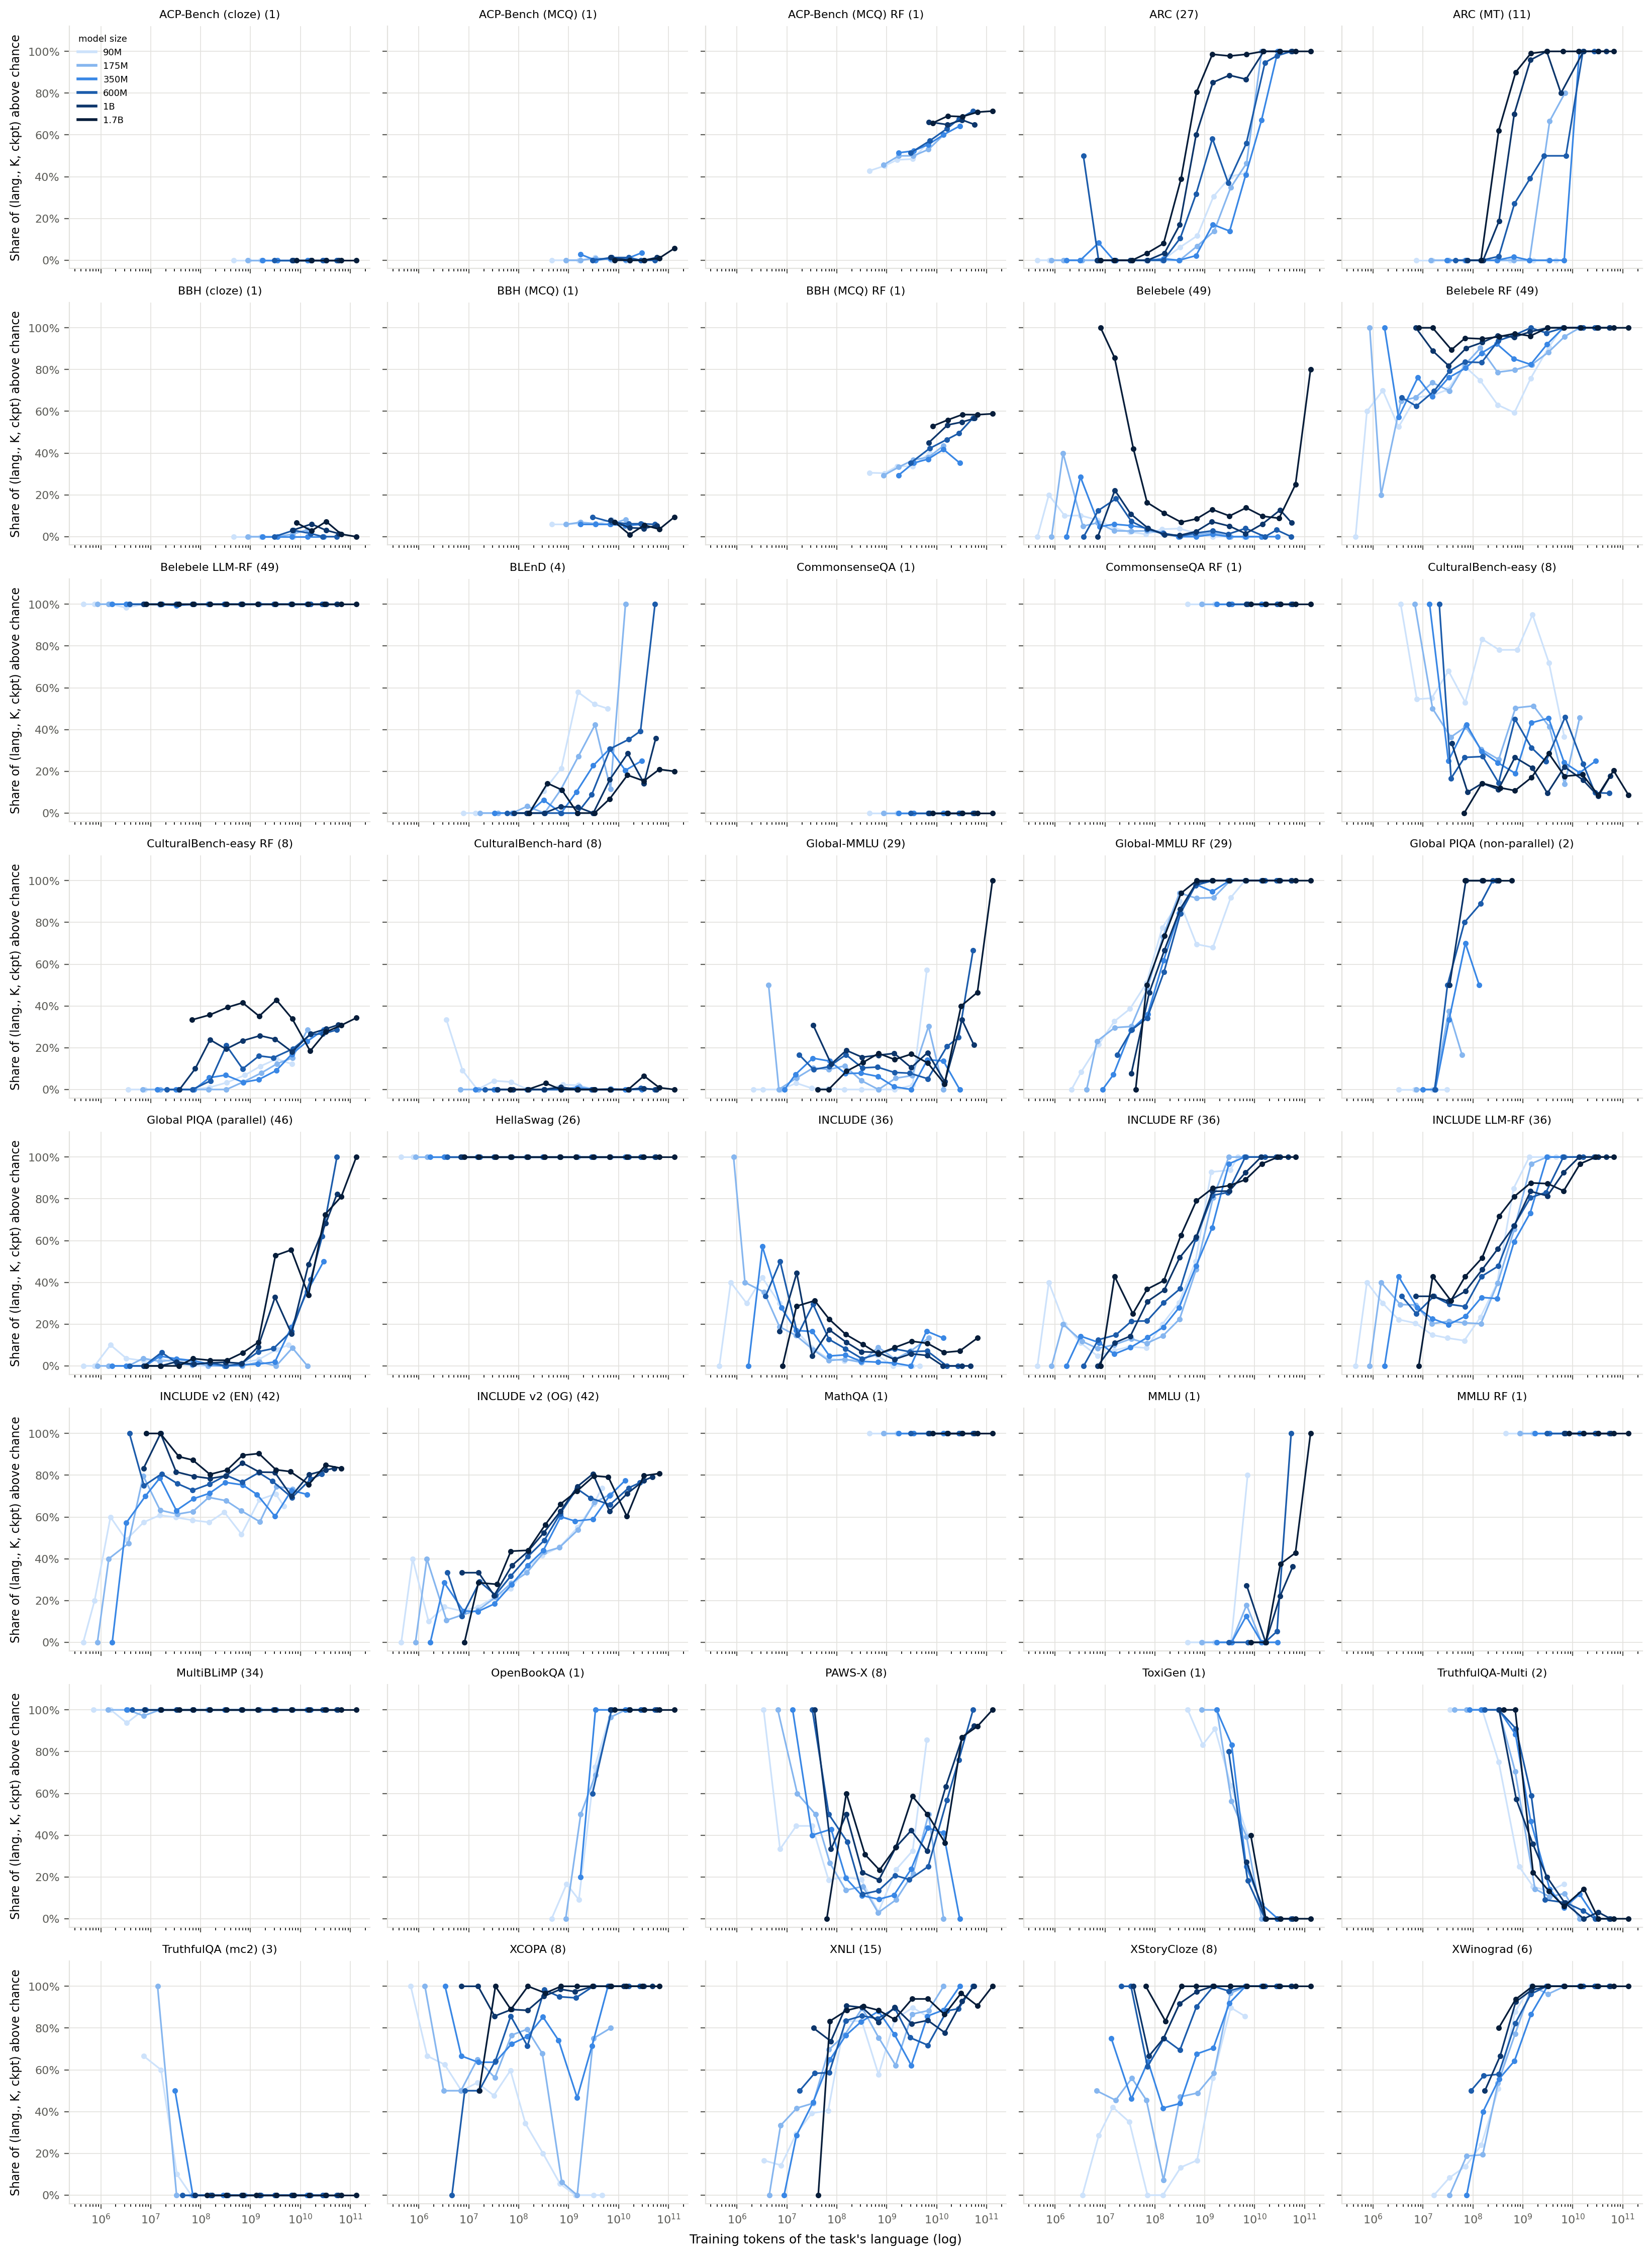
\includegraphics[width=\textwidth,height=0.8\textheight,keepaspectratio]{figures/app_rq00_chance_vs_train_tokens.png}
% source: src/signal-and-noise/analysis/rq00_chance_vs_train_tokens/pretraining/predictivity_seeds/pass_prob_vs_train_tokens_by_benchmark_1904_ckpts_paper.png
\caption{\textbf{Outside English, the share of cells above chance rises with every decade of the language's tokens from $10^{7}$ on.} One panel per benchmark (its number of tasks in parentheses). Each point is the share of (language, K, checkpoint) cells above chance, binned by the training tokens of the task's language that the checkpoint had seen (log scale). There is one line per model size, a darker blue for a larger size.}
\label{fig:app_rq00_chance_vs_train_tokens}
\end{figure*}
